%!TEX root = ../thesis.tex
%Adding the above line, with the name of your base .tex file (in this case "thesis.tex") will allow you to compile the whole thesis even when working inside one of the chapter tex files
%: ----------------------- introduction file header -----------------------
\chapter{Introduction}
\label{chap:1}


Here is the introduction of the thesis, complete with a few references  \citep{sagan1997demon, prothero2007evolution}.  Section \ref{sec:1} contains Equation \ref{eqn:1}, Section \ref{sec:2} has Figure \ref{fig:1} and Section \ref{sec:3} has Table \ref{tab:1}. Chapter \ref{chap:2} has pretty much nothing in it.

\section{First Section}\label{sec:1}
This section has an equation. Here it is:
\begin{equation}
L_{\odot} = 4\pi R_{\odot}^2 \sigma T_{e}^{4}
\label{eqn:1}
\end{equation}
which is a nice way of describing the luminosity. 

 

\section{Second Section}\label{sec:2}

So this section has a figure in it\footnote{And also a footnote.}. That figure depicts the basic structure of a red giant. 
\begin{figure}[ht!]
\includegraphics[width=\textwidth]{writeup_images/c_carma_s2.eps}
\caption[Red Giant and Asymptotic Giant Branch Stars]
%Putting the name here in square brackets won't show up in the text but will show up as the name of the figure in the list of figures at the start of the thesis
{Red Giant and Asymptotic Giant Branch Stars. The left side of the figure shows the basic structure of a star on the giant branch of the HR diagram, while the right side shows a similar star after it has evolved to ascend the asymptotic giant branch. \emph{Image Credit: Australian Telescope National Facility.}
\label{fig:1}}
\end{figure}

\section{Second Section}\label{sec:3}

